\subsubsection{Typische Komponenten und Bauweisen analoger Computer}

Der Operationsverstärker gilt als zentraler Baustein für die meisten Komponenten eines analogen Rechners. Er bildet die Differenz aus zwei Eingangssignalen und verstärkt dieses Signal anschließend. Werden ein freies und ein geerdetes Eingangssignal genutzt, so wird nur das Freie verstärkt. Durch ein Rückkopplungs-Signal gelingt es dem Operationsverstärker einen Teil der Stromverstärkung aufzugeben, um Stabilität zu gewinnen. Dieses Signal verbindet die Ausgabe der Komponente mit seiner Eingabe, wobei diese beiden Werte miteinander summiert werden. Ein wichtiges Merkmal dieser Komponente ist außerdem, dass das Vorzeichen der Eingabe gedreht wird. \cite[vgl. S. 73 f.]{Ulmann2022}

\begin{figure}[h]
  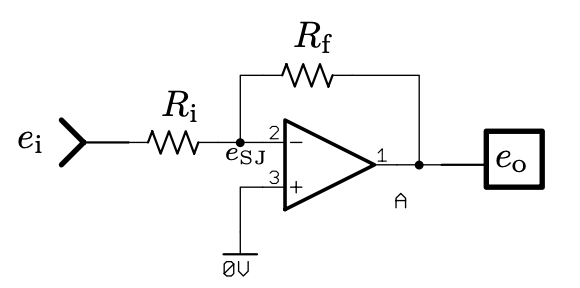
\includegraphics[width=0.5\textwidth]{abbildungen/opamp_mit_rueckkopplung.png}
  \caption{Operationsverstärker mit Rückkopplung. Quelle: \cite[S. 76]{Ulmann2022}}
  \label{fig:Operationsverstärker mit Rückkopplung}
\end{figure}

Die Formel zu Berechnung der Ausgangsspannung lautet damit wie folgt:

\[e_o=\frac{R_f}{R_i}e_i\]

Durch Anpassungen des Eingangssignals bzw. des Rückkopplungs-Signals kann die Funktion des Operationenverstärker geändert werden. So sind hiermit Operationen wie Summieren, Subtrahieren, Invertieren, das Multiplizieren von Konstanten, Integration und (bedingt) die Differenzierung möglich.

Im Prozess der Verstärkung der Signale kann ein sog. \gls{drift} auftreten. Dadurch werden kleine Fehler in der Signalverarbeitung verstärkt und führen zu großen Fehlern am Ausgang. Dieses Problem kann durch Drift-Stabilisierung gelöst werden, wie beschrieben in einem Patent von \cite{Goldberg1954}. Das durch Drift verursachte Fehlersignal kann an der Summe des Eingangs- und Rückkopplungs-Signals ausgelesen werden. Es wird verstärkt und als weiteres Eingangssignal genutzt. Somit wird der \gls{drift} ausgeglichen. \cite[vgl. S. 80]{Ulmann2022}

Um einen Summierer zu bilden, muss lediglich ein weiteres Eingangssignal zum Operationenverstärker hinzugefügt werden. Die Widerstände \(R_i\) bilden die Koeffizienten der Eingangssignale. Der Summierer bildet also die gewichtete Summe der Eingangssignale und gibt diese invertiert aus. \cite[vgl. S. 86]{Ulmann2022}

Wird der Feedback-Widerstand \(R_f\) durch einen Kondensator \(C\) ersetzt, so wird die Summe der Eingangssignale über Zeit integriert. Man erhält also einen Integrierer. Durch ein Steuerelement \textit{IC} wird ein Initialwert festgelegt, der solange ausgegeben wird, bis ein weiteres Steuerelement \textit{OP} betätigt wird. Im aktivierten Zustand wird solange das Integral der Eingangssignale ausgegeben, bis der \textit{OP} Schalter erneut betätigt wird und der letzte gespeicherte Wert ausgegeben wird. \cite[vgl. S. 89 ff.]{Ulmann2022}

Die Anwendung eines Koeffizienten am Operationenverstärker kann durch ein Potentiometer erfolgen, welches am Eingangssignal angeschlossen ist. Das somit erhaltene Koeffizient-Potentiometer lässt sich über einen speziellen Zustand des Analogrechners, dem \textit{Potentiometer Set} (kurz: \textit{Pot Set}) setzen. In diesem Zustand werden alle Recheneinheiten des Analogrechners deaktiviert, sodass das rohe Eingangssignal weitergeleitet wird. In großen analogen Rechnern werden Potentiometer durch Servomotoren oder in hybriden Rechnern digital gesteuert. \cite[vgl. S. 92 ff.]{Ulmann2022}

Ein Funktionsgenerator kann genutzt werden, um eine beliebige Funktion \(f(x,...)\) abzubilden. Für analoge Rechner ist das aber eine komplexe Aufgabe, weshalb sich für diesen Anwendungsfall hybride Systeme besonders eignen. Als mögliche analoge Ansätze bieten sich der servogetriebene Funktionsgenerator, der Kurvenfolger oder der Fotoformer an. \cite[vgl. S. 97 ff.]{Ulmann2022}

Die im ersten Augenblick einfache Multiplizierung ist auf analogen Rechnern komplex zu implementieren \cite[vgl. S. 105]{Ulmann2022}. Moderne analoge Rechner greifen typischerweise auf die Gilbert Zelle zurück (TODO: Quellenangabe). Die Berechnung einer Division bzw. Quadratwurzel kann durch modifizierte Multiplikatoren erfolgen. \cite[S. 114 f.]{Ulmann2022}

Ein Komparator kann z.B. zur Implementierung einer Schrittfunktion oder zum Tauschen von Variablen genutzt werden. Um das zu erreichen reicht es schon aus, Dioden in der Feedback-Schleife eines Operationenverstärkers zu platzieren. Nach einem ähnlichen Prinzip kann auch ein Begrenzer erzeugt werden, dessen Eingangssignal zwischen einer Ober- und Untergrenze limitiert wird. \cite[S. 116]{Ulmann2022}
